\documentclass[ignoreframetext]{beamer}
\usepackage[utf8]{inputenc}
\usepackage[T1]{fontenc}
\usepackage[british]{babel}
\usepackage{booktabs}

\usepackage[all]{foreign}
\renewcommand{\foreignfullfont}{}
\renewcommand{\foreignabbrfont}{}

\usepackage{newclude}
\usepackage{import}

\usepackage[strict]{csquotes}
\usepackage[single]{acro}

\usepackage[natbib,style=alphabetic,maxbibnames=99]{biblatex}
\addbibresource{bibedu.bib}

\usepackage{subcaption}

\usepackage[noend]{algpseudocode}
\usepackage{xparse}

\let\email\texttt

\usepackage[outputdir=ltxobj]{minted}
\setminted{autogobble}

\usepackage{amsmath}
\usepackage{amssymb}
\usepackage{mathtools}
\usepackage{amsthm}
\usepackage{thmtools}
\usepackage[unq]{unique}
\DeclareMathOperator{\powerset}{\mathcal{P}}

\usepackage[binary-units]{siunitx}

\usepackage[capitalize]{cleveref}

\newcommand\hitem{%
  \leavevmode%
  {\usebeamercolor[fg]{structure}%
  \usebeamertemplate{itemize item}}\hspace{0.5em}%
}


\usetheme{Berlin}
\setbeamertemplate{footline}%{miniframes theme}
{%
  \begin{beamercolorbox}[colsep=1.5pt]{upper separation line foot}
  \end{beamercolorbox}
  \begin{beamercolorbox}[ht=2.5ex,dp=1.125ex,%
    leftskip=.3cm,rightskip=.3cm plus1fil]{author in head/foot}%
    \leavevmode{\usebeamerfont{author in head/foot}\insertshortauthor}%
    \hfill%
    {\usebeamerfont{institute in head/foot}\usebeamercolor[fg]{institute in head/foot}\insertshortinstitute}%
  \end{beamercolorbox}%
  \begin{beamercolorbox}[ht=2.5ex,dp=1.125ex,%
    leftskip=.3cm,rightskip=.3cm plus1fil]{title in head/foot}%
    {\usebeamerfont{title in head/foot}\insertshorttitle} \hfill     \insertframenumber%
  \end{beamercolorbox}%
  \begin{beamercolorbox}[colsep=1.5pt]{lower separation line foot}
  \end{beamercolorbox}
}
\setbeamercovered{transparent}
\setbeamertemplate{bibliography item}[text]

\AtBeginSection[]{%
  \begin{frame}<beamer>
    \tableofcontents[currentsection]
  \end{frame}
}

\ProvideDocumentEnvironment{assumption}{o}{%
  \IfValueTF{#1}{%
    \begin{block}{Assumption: #1}
  }{%
    \begin{block}{Assumption}
  }
}{%
  \end{block}
}

\ProvideDocumentEnvironment{protocol}{o}{%
  \IfValueTF{#1}{%
    \begin{block}{Protocol: #1}
  }{%
    \begin{block}{Protocol}
  }
}{%
  \end{block}
}

\ProvideDocumentEnvironment{remark}{o}{%
  \IfValueTF{#1}{%
    \begin{alertblock}{Note: #1}
  }{%
    \begin{alertblock}{Note}
  }
}{%
  \end{alertblock}
}

\ProvideDocumentEnvironment{idea}{o}{%
  \IfValueTF{#1}{%
    \begin{block}{Idea: #1}
  }{%
    \begin{block}{Idea}
  }
}{%
  \end{block}
}

\ProvideDocumentEnvironment{question}{o}{%
  \setbeamercolor{block body}{bg=orange!15,fg=black}
  \setbeamercolor{block title}{bg=orange,fg=white}
  \setbeamercolor{local structure}{fg=orange}
  \IfValueTF{#1}{%
    \begin{block}{Question: #1}
  }{%
    \begin{block}{Question}
  }
}{%
  \end{block}
}

\ProvideDocumentEnvironment{exercise}{o}{%
  \setbeamercolor{block body}{bg=yellow!10,fg=black}
  \setbeamercolor{block title}{bg=yellow,fg=black}
  \setbeamercolor{local structure}{fg=yellow}
  \IfValueTF{#1}{%
    \begin{block}{Exercise: #1}
  }{%
    \begin{block}{Exercise}
  }
}{%
  \end{block}
}


\begin{document}
\title{%
  Reflections on Necessary Conditions of Learning:
  Cherry Picking
}
\author{Daniel Bosk}
\institute{%
  KTH EECS
}

\begin{frame}
  \maketitle
\end{frame}

\mode<all>
\mode*

\section{Introduction}

\subsection{The book and author}

\begin{frame}
  \begin{figure}
    
\includegraphics[height=0.8\textheight]{fig/book.jpg}
    \caption{Front cover of Necessary Conditions of Learning.}
  \end{figure}
\end{frame}

\begin{frame}
  \begin{figure}
    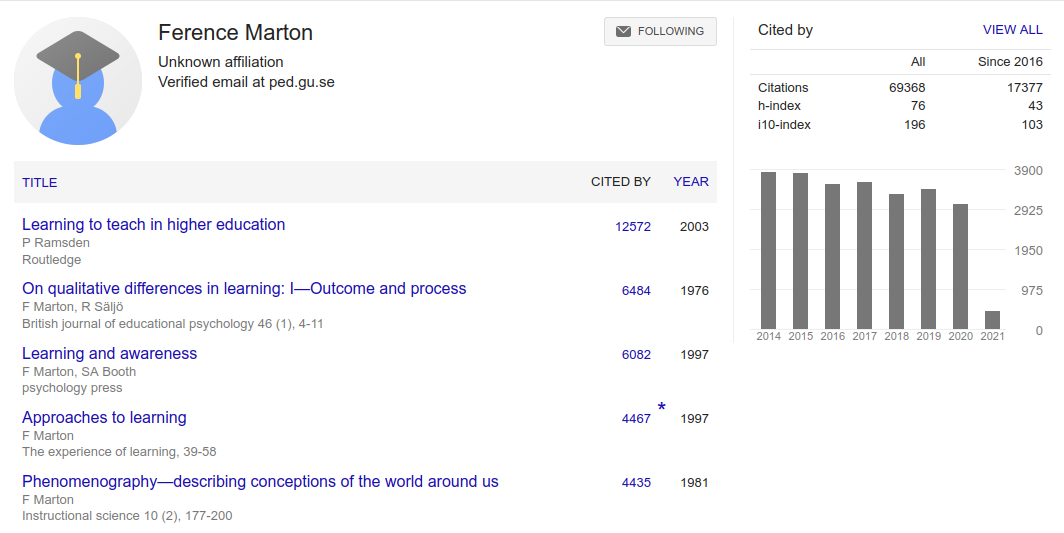
\includegraphics[width=\columnwidth]{fig/marton-gscholar.png}
    \caption{Marton's profile on Google Scholar, showing his high citation 
    counts.}
  \end{figure}
\end{frame}

\begin{frame}
  \begin{figure}
    
\includegraphics[width=\columnwidth]{fig/necessary-conditions-citations.png}
    \caption{Citations for the book.}
  \end{figure}
\end{frame}

\begin{frame}
  \begin{block}{Main ideas}
    \begin{itemize}
      \item Phenomenography~\cite{Phenomenography}
      \item Variation theory~\cite{VariationTheory}
      \item Learning studies~\cite{LearningStudy}
    \end{itemize}
  \end{block}
\end{frame}

\subsection{Phenomenography}

\begin{frame}
  \blockcquote{NecessaryConditionsOfLearning}{%
    We tacitly assume that what we see is exactly what is there to be seen and 
    that others see things in the same way we do. It is hard to realize that we 
    have actually learned to see the world in certain ways and that others may 
    have learned to see it differently.
  }
\end{frame}

\begin{frame}
  \begin{block}<1-2>{Phenomenography~\cite{Phenomenography}}
    \begin{itemize}
      \item Reality is experienced.
      \item People interpret significant aspects of reality.
    \end{itemize}
    \pause
    \begin{description}
      \item[First-order perspective] describes various aspects of the world.
      \item[Second-order perspective] describes people's experiences of various 
        aspects of the world --- phenomenography.
    \end{description}
  \end{block}
\end{frame}

\subsection{Variation theory}

\begin{frame}
  \begin{block}{Variation theory~\cite{VariationTheory}}
    \vspace{-0.5em}
    \[
      \text{learning}
      \quad\leftarrow\quad
      \text{discernment}
      \quad\leftarrow\quad
      \text{variation}
    \]
  \end{block}

  \pause

  \begin{remark}
    \begin{itemize}
      \item There must be a pattern of variation to experience.
      \item \emph{This pattern must be experienced}.
    \end{itemize}
  \end{remark}
\end{frame}

\begin{frame}
  \begin{block}{Patterns of variation}
    \vspace{-0.5em}
    \[
      \text{contrast}
      \quad\rightarrow\quad
      \text{generalization}
      \quad\rightarrow\quad
      \text{fusion}
    \]
  \end{block}

  \begin{figure}
    \begin{subfigure}{0.3\columnwidth}
      \centering
      \begin{tikzpicture}
        \fill[blue] (-0.75, 0) circle (0.5);
        \fill[green] (0.75, 0) circle (0.5);
      \end{tikzpicture}
      \caption{Contrast}
    \end{subfigure}
    \hfill
    \begin{subfigure}{0.3\columnwidth}
      \centering
      \begin{tikzpicture}
        \fill[blue] (-0.75, 0) circle (0.5);
        \fill[blue] (0.5, -0.5) rectangle (1.5, 0.5);
      \end{tikzpicture}
      \caption{Generalization}
    \end{subfigure}
    \hfill
    \begin{subfigure}{0.3\columnwidth}
      \centering
      \begin{tikzpicture}
        \fill[orange] (-0.75, 0) circle (0.5);
        \fill[purple] (0.5, -0.5) rectangle (1.5, 0.5);
      \end{tikzpicture}
      \caption{Fusion}
    \end{subfigure}
    \caption{%
      Illustrating the patterns of variation for aspects color and shape.
    }
  \end{figure}
\end{frame}

\begin{frame}
  \begin{figure}
    \semitransp{%
      \begin{subfigure}{0.3\columnwidth}
        \centering
        \begin{tikzpicture}
          \fill[blue] (-0.75, 0) circle (0.5);
          \fill[green] (0.75, 0) circle (0.5);
        \end{tikzpicture}
        \caption{Contrast}
      \end{subfigure}
    }
    \hfill
    \begin{subfigure}{0.3\columnwidth}
      \centering
      \begin{tikzpicture}
        \fill[blue] (-0.75, 0) circle (0.5);
        \fill[blue] (0.5, -0.5) rectangle (1.5, 0.5);
      \end{tikzpicture}
      \caption{Generalization}
    \end{subfigure}
    \hfill
    \semitransp{%
      \begin{subfigure}{0.3\columnwidth}
        \centering
        \begin{tikzpicture}
          \fill[orange] (-0.75, 0) circle (0.5);
          \fill[purple] (0.5, -0.5) rectangle (1.5, 0.5);
        \end{tikzpicture}
        \caption{Fusion}
      \end{subfigure}
      \caption{%
        Illustrating the patterns of variation for aspects color and shape.
      }
    }
  \end{figure}

  \begin{remark}
    \begin{itemize}
      \item We tend to focus on generalization/induction.
      \item \enquote{Good theses from previous years.}
      \item \enquote{One example of linear function, another example of linear 
        function.}
    \end{itemize}
  \end{remark}
\end{frame}

\subsection{Learning study}

\begin{frame}
  \begin{block}{Learning study~\cite{LearningStudy}}
    \begin{itemize}
      \item Design-Based Research + Variation Theory
      \item Extends the Japanese concept Lesson Study.
    \end{itemize}
    \pause
    \begin{enumerate}
      \item \label{design} (Re-)Design teaching material/plan using variation 
        theory.
      \item Perform teaching.
      \item Analyze teaching performance and outcomes.
      \item Go to \ref{design}.
    \end{enumerate}
  \end{block}

  \pause

  \begin{remark}
    \begin{itemize}
      \item Teacher teams, teach the same thing to different classes.
      \item Yields iterations.
    \end{itemize}
  \end{remark}
\end{frame}

\begin{frame}
  \begin{example}
    \begin{itemize}
      \item I'll work systematically according to this with my TAs.
    \end{itemize}
  \end{example}
\end{frame}

\subsection{Disposition}

\begin{frame}
  \begin{enumerate}
    \item What makes humans human?
    \item What is to be learned?
    \item Sameness and difference in learning
    \item What does the world look like to others?
    \item The art of learning
    \item Making learning possible
    \item Learning to help others to learn
  \end{enumerate}
\end{frame}

\begin{frame}
  \begin{block}{Ch 1 What makes humans human?}
    \begin{itemize}
      \item What is pedagogy, how does it relate to learning.
    \end{itemize}
  \end{block}
\end{frame}

\begin{frame}
  \begin{block}{Ch 2 What is to be learned?}
    \begin{itemize}
      \item What is an intended learning outcome?
      \item What should it be?
      \item It depends on the learner: \emph{critical aspects, critical 
        features}.
    \end{itemize}
  \end{block}
\end{frame}

\begin{frame}
  \begin{figure}
    \begin{subfigure}{0.3\columnwidth}
      \centering
      \begin{tikzpicture}
        \fill[blue] (-0.75, 0) circle (0.5);
        \fill[green] (0.75, 0) circle (0.5);
      \end{tikzpicture}
      \caption{Contrast}
    \end{subfigure}
    \hfill
    \begin{subfigure}{0.3\columnwidth}
      \centering
      \begin{tikzpicture}
        \fill[blue] (-0.75, 0) circle (0.5);
        \fill[blue] (0.5, -0.5) rectangle (1.5, 0.5);
      \end{tikzpicture}
      \caption{Generalization}
    \end{subfigure}
    \hfill
    \begin{subfigure}{0.3\columnwidth}
      \centering
      \begin{tikzpicture}
        \fill[orange] (-0.75, 0) circle (0.5);
        \fill[purple] (0.5, -0.5) rectangle (1.5, 0.5);
      \end{tikzpicture}
      \caption{Fusion}
    \end{subfigure}
    \caption{%
      Illustrating the patterns of variation for aspects color and shape.
    }
  \end{figure}

  \begin{onlyenv}<1>
    \begin{example}
      \begin{itemize}
        \item Critical aspect: colour.
        \item Critical feature: blue.
        \item Non-critical feature: green.
        \item Non-critical aspect: shape.
        \item Non-critical features: circle, square.
      \end{itemize}
    \end{example}
  \end{onlyenv}
  \begin{onlyenv}<2>
    \begin{remark}
      \begin{itemize}
        \item There are other aspects too, \emph{unintentionally}.
        \item Another aspect in this figure is order: the circle is always 
          \enquote{first} (to the right).
      \end{itemize}
    \end{remark}
  \end{onlyenv}
\end{frame}

\begin{frame}
  \begin{figure}
    \includegraphics[height=0.5\textheight]{fig/maja-writing.png}
    \caption{My daughter's writing.}
  \end{figure}
  \begin{example}
    \begin{itemize}
      \item Obviously my daughter knows some aspect(s) of writing.
      \item Just not all that are needed.
    \end{itemize}
  \end{example}
\end{frame}

\begin{frame}
  \begin{block}{Ch 3 Sameness and difference in learning}
    \begin{itemize}
      \item The problem with direct reference.
    \end{itemize}
  \end{block}
\end{frame}

\begin{frame}
  \begin{block}{Ch 4 What does the world look like to others?}
  \end{block}
\end{frame}

\begin{frame}
  \begin{block}{Ch 5 The art of learning}
  \end{block}
\end{frame}

\begin{frame}
  \begin{block}{Ch 6 Making learning possible}
  \end{block}
\end{frame}

\begin{frame}
  \begin{block}{Ch 7 Learning to help others to learn}
  \end{block}
\end{frame}

\mode*

\begin{frame}[allowframebreaks]
  \printbibliography
\end{frame}
\end{document}
